\chapter{Readability or Understandability}

Readable code is one in which the components of the code are easy to grasp and the goal of the overall code is well defined. Building a codebase that is readable is not just a single goal for a team but a commitment that lasts the entire duration of the project. Developers should think of themselves as authors of their code instead of configuration of a complex piece of software.

Here are some cultural habits that leads to a readable code:


\begin{itemize}
  \item A good code review practice is in place and rules are set from the onset of the project.
  \item Developers are mindful of how someone new will perceive their code.
  \item The Boy Scout Rule - "Leave the campground cleaner than you found it" is followed which iteratively improves the readability of code.
\end{itemize}



\section{Well formatted and follows standards}

Every popular language/framework has guidelines over how code should be formatted and a list of dos and don'ts. It is best to start with these standards at the onset of the project. Sometimes the team may have custom stylistic preferences. These should be well documented and people from outside the team may not follow these standards. Also, it is important to not overstretch the standards as this makes documenting and enforcing standards a burden in itself. As it could be a tedious process to monitor, evaluate and enforce the standards, most teams use linters and prettifiers. Additionally, standard code quality analyzer tools like Sonarqube and Codeclimate can dramatically improve the code review process through automation. It is highly recommended that projects mandate usage of these tools.


\section{Right documentation}
It is popularly said that good code is self documented. While code should definitely have inherent readable qualities, it is wishful thinking to rely on this alone. Just like coding skills, documentation skills can be developed through learning and practice. Developers are recommended to learn about documentation syntaxes and standards for their respective frameworks. Expertise in Docblocks, knowledge of Markdown, RST or alike, and of diagram tools such as draw.io, lucidcharts etc help in producing crisp documentation. A project can also start using automatic documentation generation tools of their liking.

\section{Convention over configuration}

Conventions such as naming and placement of artifacts increase the readability of code in two ways. First, they enforce a high degree of consistency, and second they eliminate the burden of thinking about what parameters needs to be set in a configuration file.

To take this a step further is to create structures such as Abstract classes, Enumerations and choose a logic organization strategy such as MVC (Model View Controller)

\section{Libraries}
It is advised to practice restraint on picking libraries. We can run into libraries that fully solve our problems but are obscure, and there are ones that partially solve our problems that are very popular. 

Writing one's own library can sometimes seem tempting and can be beneficial as the end product is tailored to the project's needs and is fully under the developer's control. However, with the power also comes the necessity to maintain and document the workings of the library. Libraries which are publicly available do not necessitate this as the documentation and maintenance is performed by the owner or the community.
 
\section{Zen of Python}

Although this topic might look like it’s specific to Python, you will find it useful across all languages and platforms. Like “Zen Religion”, you will find that many things in this guideline is not absolute and is open to interpretation

\begin{center}
	\makebox[0.95\textwidth]{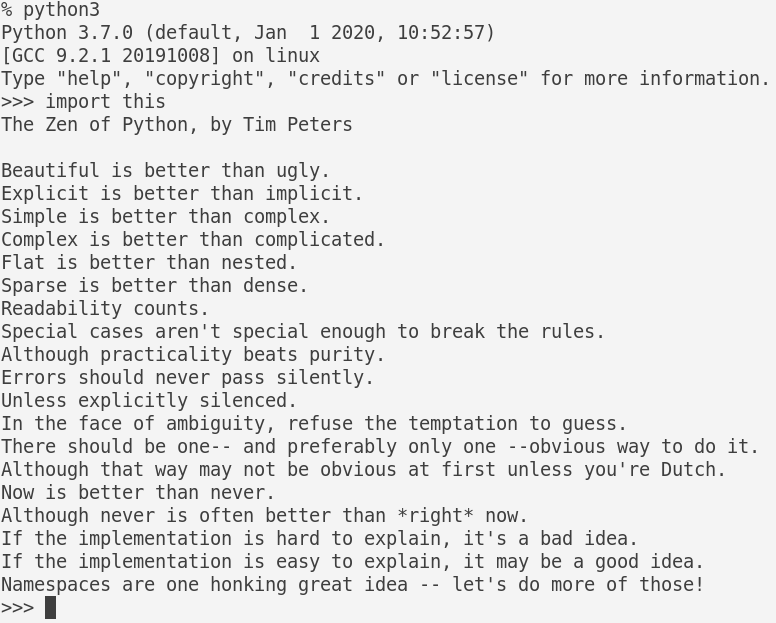
\includegraphics[width=0.95\textwidth]{readability_or_understandability/zen_of_python.png}}
\end{center}


\section{Useful Patterns}

Some other ways to increase readability of code are as follows:

\begin{itemize}
  \item Use Objects, Maps or Dictionaries instead of too many conditionals.
  \item Use Programmable objects in representing APIs such as the ones provided by ORMs.
  \item Naming should be consistent across variables, functions, files, database artifacts etc. For example, having a consistent style of prefixing such as "is\_" prefix for booleans, "on\_" prefix for callbacks, "view\_" prefix for views etc can enhance readability 
  \item Write functions that have a single responsibility. Avoid writing functions with side-effects.
  \item Focus on tests as tests such as unit tests to improve code quality as well as readability
\end{itemize}

